% =====================================================================
%  ANCHOR — A1 BETTER POSTER (landscape)
%
%  Three-column layout:
%    Left   (~22%, cream):   title, authors, BACKGROUND / APPROACH /
%                            OUTCOMES / LINEAGE.
%    Centre (~56%, flat dark teal): logos, big takeaway, subline,
%                            funding footer.
%    Right  (~22%, cream):   graphical-abstract slot, WHAT INDUSTRY
%                            GETS, READ MORE + QR.
%
%  Compile with XeLaTeX:
%      latexmk better-poster.tex
% =====================================================================

\documentclass{article}

\usepackage[paperwidth=841mm, paperheight=594mm,
            margin=0pt, noheadfoot]{geometry}
\usepackage{fontspec}
\usepackage{xcolor}
\usepackage{graphicx}
\usepackage{tikz}
\usetikzlibrary{shadows}
\usepackage[absolute, overlay]{textpos}
\usepackage{ragged2e}
\usepackage{microtype}
\usepackage[hidelinks]{hyperref}
\usepackage{qrcode}

% Fonts
\setmainfont{Open Sans}
\newfontfamily\headingfont{Montserrat}
\newfontfamily\titlefont{Montserrat ExtraBold}
\newfontfamily\bigfont{Montserrat Black}
\setmonofont{Inconsolata}

% Colour palette — Anchor is the warm-orange sibling of the yellow PhD posters
\definecolor{paneltext}{HTML}{1B1B1B}
\definecolor{panelbg}{HTML}{F2EFE8}     % warm cream for side panels
\definecolor{panelmuted}{HTML}{6E6E6E}  % muted body grey
\definecolor{centerbg}{HTML}{0F3438}    % flat dark teal centre band
\definecolor{centertext}{HTML}{FFFFFF}
\definecolor{centermuted}{HTML}{B8C9CB} % muted text on dark teal
\definecolor{accent}{HTML}{FF8E2B}      % warm orange highlight
\definecolor{slotborder}{HTML}{C9C2B4}  % dashed border for the figure slot

% TextPos in mm
\setlength{\TPHorizModule}{1mm}
\setlength{\TPVertModule}{1mm}
\textblockorigin{0mm}{0mm}

\graphicspath{{../assets/}{assets/}{screenshots/}{figures/}{generated/}{./}}

\pagestyle{empty}
\setlength{\parindent}{0pt}
\setlength{\parskip}{0.55\baselineskip}
\linespread{1.18}

% Column geometry (mm). Landscape A1: 22/56/22 split of 841 mm width.
\newcommand{\leftColW}{185}
\newcommand{\centerColX}{185}
\newcommand{\centerColW}{471}
\newcommand{\rightColX}{656}
\newcommand{\rightColW}{185}
\newcommand{\panelPad}{14}
\newcommand{\barH}{55}         % black title bar across the top (mm)
\newcommand{\contentTop}{60}   % where content starts below the bar

% Side-panel section heading
\newcommand{\panelhead}[1]{%
  \par\addvspace{5mm}%
  {\headingfont\bfseries\fontsize{14pt}{17pt}\selectfont
   \MakeUppercase{#1}\par}%
  \nopagebreak\vspace{1mm}%
  \textcolor{accent}{\rule{32mm}{1.5pt}}\par
  \vspace{1.5mm}%
}

% Highlight a phrase inside the big takeaway
\newcommand{\hl}[1]{\textcolor{accent}{#1}}

% Arrow that renders in any font (Open Sans Regular lacks U+2192).
\newcommand{\arr}{\ensuremath{\rightarrow}}

\begin{document}

% ---------------------------------------------------------------------
%  BACKGROUND PANELS
% ---------------------------------------------------------------------
\begin{tikzpicture}[remember picture, overlay]
  % --- BLACK TITLE BAR across the full width at the very top ---------
  % Sub-hero: gives identity at a glance, but the centre takeaway
  % below is still the visual heavyweight (better-poster ideology).
  \fill[black]
     (current page.north west)
     rectangle
     ([yshift=-\barH mm]current page.north east);

  % --- Left & right cream panels (start below the bar) ---------------
  \fill[panelbg]
     ([yshift=-\barH mm]current page.north west)
     rectangle
     ([xshift=\leftColW mm]current page.south west);
  \fill[panelbg]
     ([xshift=\rightColX mm, yshift=-\barH mm]current page.north west)
     rectangle
     (current page.south east);

  % --- Centre band: cruise_grad.png (starts below the bar) -----------
  % Image is 2250×4000 px; new band aspect = 471/(594-55) = 471/539
  % ≈ 0.874 → keep a 2250×2575 strip. Anchor to the bottom of the
  % source so the darkest sea lands at the bottom of the column where
  % the funding line sits.
  \node[anchor=north west, inner sep=0pt]
     at ([xshift=\centerColX mm, yshift=-\barH mm]current page.north west)
     {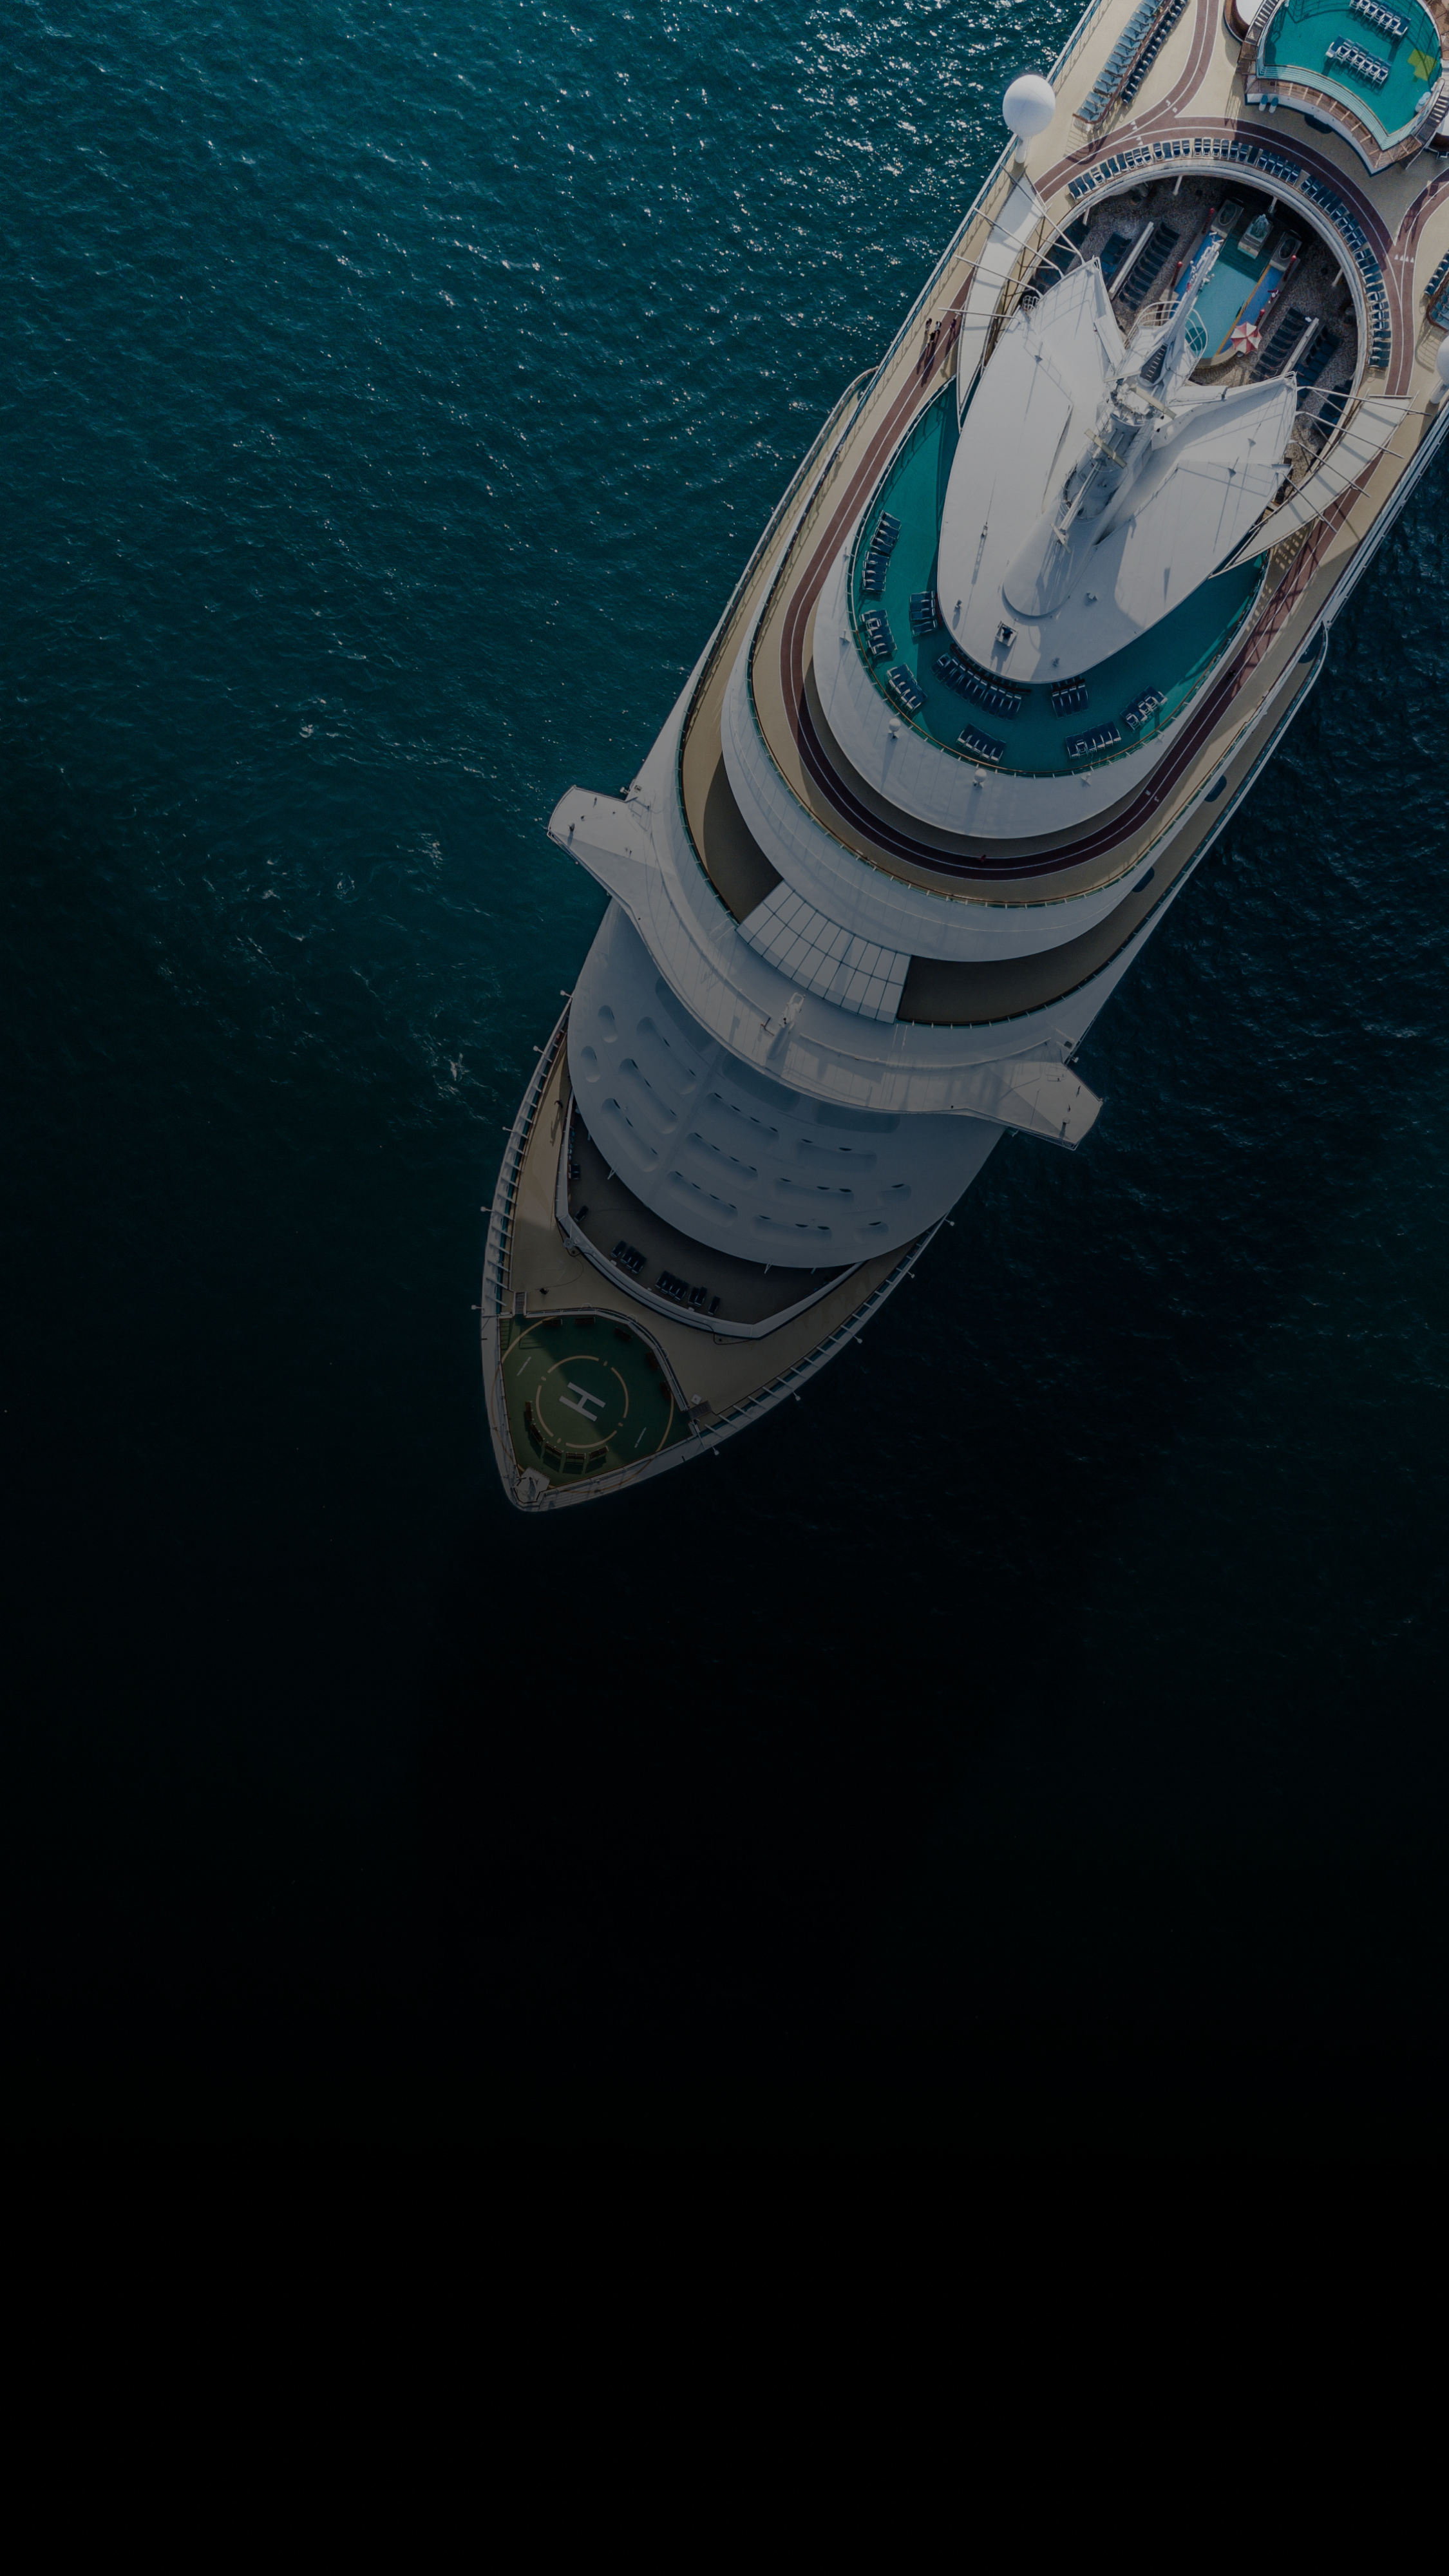
\includegraphics[width=\centerColW mm,
                       viewport=0 0 2250 2575, clip]{cruise_grad.png}};
\end{tikzpicture}

% ---------------------------------------------------------------------
%  TOP BAR — Anchor mark + wordmark + tagline / Novia logo
% ---------------------------------------------------------------------
% Left side of the bar: logo mark + wordmark + tagline.
\begin{textblock}{600}(20,8)
  \color{centertext}
  \begin{minipage}[c]{\linewidth}
    
\includegraphics[height=36mm]{anchor-white.pdf}\hspace{6mm}%
    \raisebox{6mm}{%
      \begin{minipage}[b]{0.78\linewidth}
        {\headingfont\bfseries\fontsize{52pt}{52pt}\selectfont Anchor\par}
        \vspace{2mm}
        {\headingfont\fontsize{14pt}{17pt}\selectfont
         % Two MCP tools. Datasheets in, grounded answers out.
         Datasheets in. Page-grounded answers out.\par}
      \end{minipage}}%
  \end{minipage}
\end{textblock}

% Right side of the bar: Novia logo (white, on black). Anchor poster
% uses Novia only — no ÅA logo on this one.
\begin{textblock}{160}(665,17)
  \color{centertext}\hfill
  
\includegraphics[height=30mm]{logoinvinternwhite.pdf}\hfill\strut
\end{textblock}

% ---------------------------------------------------------------------
%  LEFT COLUMN — authors + paper-style content
% ---------------------------------------------------------------------
\begin{textblock}{157}(14,\contentTop)          % 185 - 2*14 = 157 mm wide
  \color{paneltext}\fontsize{11pt}{15pt}\selectfont\RaggedRight

  {\linespread{1}\fontsize{9.5pt}{11.5pt}\selectfont
   \textbf{Christoffer Björkskog} · christoffer.bjorkskog@novia.fi\par
   \textbf{Lamin Jatta} · lamin.jatta@novia.fi\par
   Maritime Technology, Novia University of Applied Sciences\par
   \vspace{0.8mm}
   \textbf{Supervisors:} Andreas Lundell (ÅAU),
   Johan Westö (Novia UAS), Mikael Manngård (Novia UAS).\par}

  \panelhead{Problem}
  AI is already part of engineering work and won't go away. But facts without a clear
  source can't be trusted, and shouldn't be. Verifying each claim by opening PDFs
  and scrolling defeats the speed AI was supposed to give.

  \panelhead{What is Anchor}
  Anchor is a tool for working with engineering documents. From a PDF datasheet, an FMU, a CAD file, or anything else exposed through the Open Ingestion Protocol (OIP), Anchor ingests it and
  extracts the parts (spec rows, charts, ports, parameters) and makes each one independently addressable by humans and AI agents. Every value keeps a reference back to where it came
  from in the source. Anchor ships wtih support for PDF, and FMU ingestion, whereas CAD and SysML extensions are under development.

  \panelhead{Ingestion}
  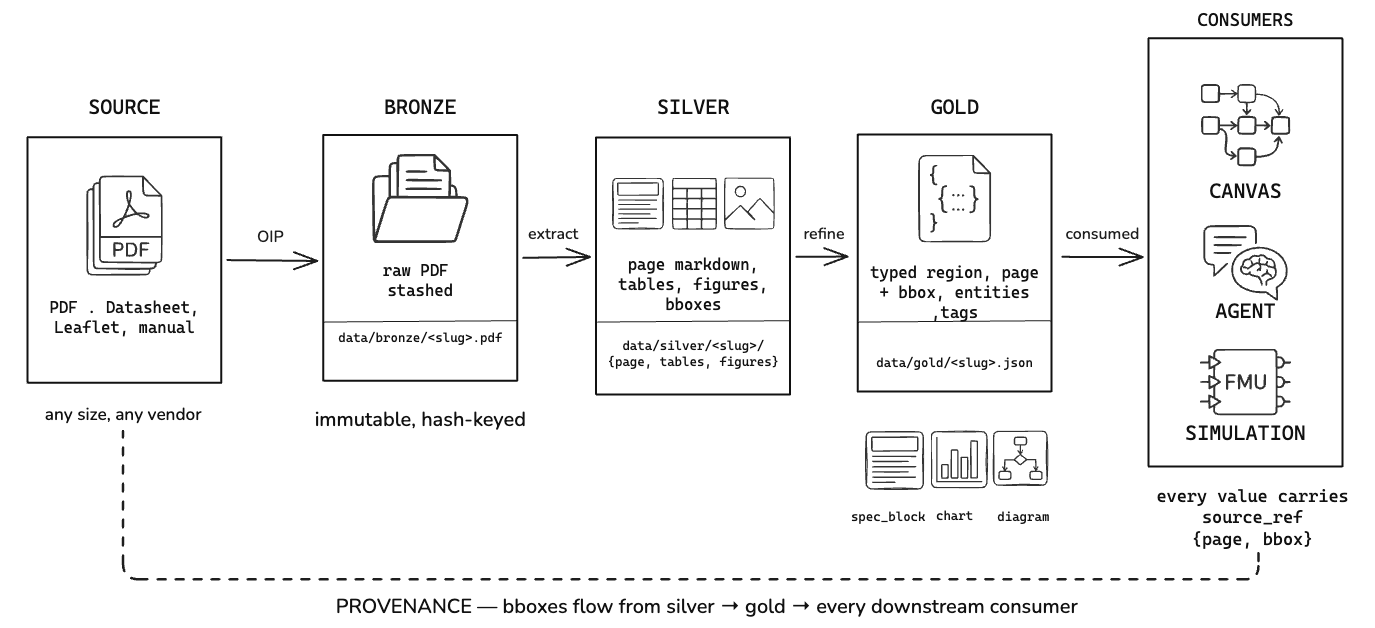
\includegraphics[width=\linewidth]{ingestion-vector.png}
  \vspace{1mm}
  {\fontsize{8.5pt}{11pt}\selectfont\color{panelmuted}
  A vision-LLM region-extraction step at gold keeps each region semantically
  coherent: a table header stays with its table, a spec block stays whole.
  Every value flows forward with its source page and bbox.\par}

  \panelhead{Built}
  \begin{itemize}\setlength{\itemsep}{1.5pt}\setlength{\parsep}{1pt}\setlength{\leftmargin}{4mm}
    \item Engineering PDFs go through bronze \arr{} silver \arr{} gold with a vision-LLM region polish; an FMU extension ships alongside as an example for other source kinds.
    \item MCP tools cover canvas commands and each producer's actions, namespaced (\texttt{pdf.*}, \texttt{fmu.*}, \dots) so producers coexist.
    \item Generic node types (concept, entity, fact, document, spec, area, note) ship built-in; extensions register their own renderers at runtime.
    \item Pure domain core with HTTP, MCP, and a CLI as peer adapters; import-linter contracts keep the boundaries clean in CI. Vendor SDKs live only in extension infra; the core never sees them.
    \item JSONL event log per workspace; plain-file artefacts per document. No database, no queue. Multi-client sync ($\sim$50\,ms) is a side effect of the in-memory bus.
  \end{itemize}

  \panelhead{Portable}
  A canvas is a folder: events.jsonl plus a derived snapshot. Tar it, copy it to
  another machine, replay; same state, same provenance. Audit, time-travel, and
  migration are mechanical, not features that have to be added.

  \vfill
  {\color{panelmuted}\fontsize{8.5pt}{11pt}\selectfont
   Novia University of Applied Sciences\par}
\end{textblock}

% ---------------------------------------------------------------------
%  CENTRE COLUMN — big takeaway, flow strip, footer
%  (Project identity + logos now live in the top bar.)
% ---------------------------------------------------------------------

% BIG TAKEAWAY — sits over the dark sea below the cruise ship deck
\begin{textblock}{443}(199,205)
  \color{centertext}\centering
  {\bigfont\fontsize{72pt}{86pt}\selectfont
   Every spec your agent quotes\\
   points back to the\\
   \hl{page it came from}.\par}
  \vspace{10mm}
  {\headingfont\fontsize{22pt}{28pt}\selectfont
   Datasheet \arr{} canvas \arr{} simulation.\\
   Each step keeps the source.\par}
\end{textblock}

% --- ARCHITECTURE DIAGRAM on the dark sea, below the takeaway --------
% Hand-drawn-style figure from paperx/figures/architecture.png.
% Black-on-black aesthetic merges with the dark sea backdrop. Centred
% horizontally in the centre column.
\begin{textblock}{443}(199,355)
  \centering
  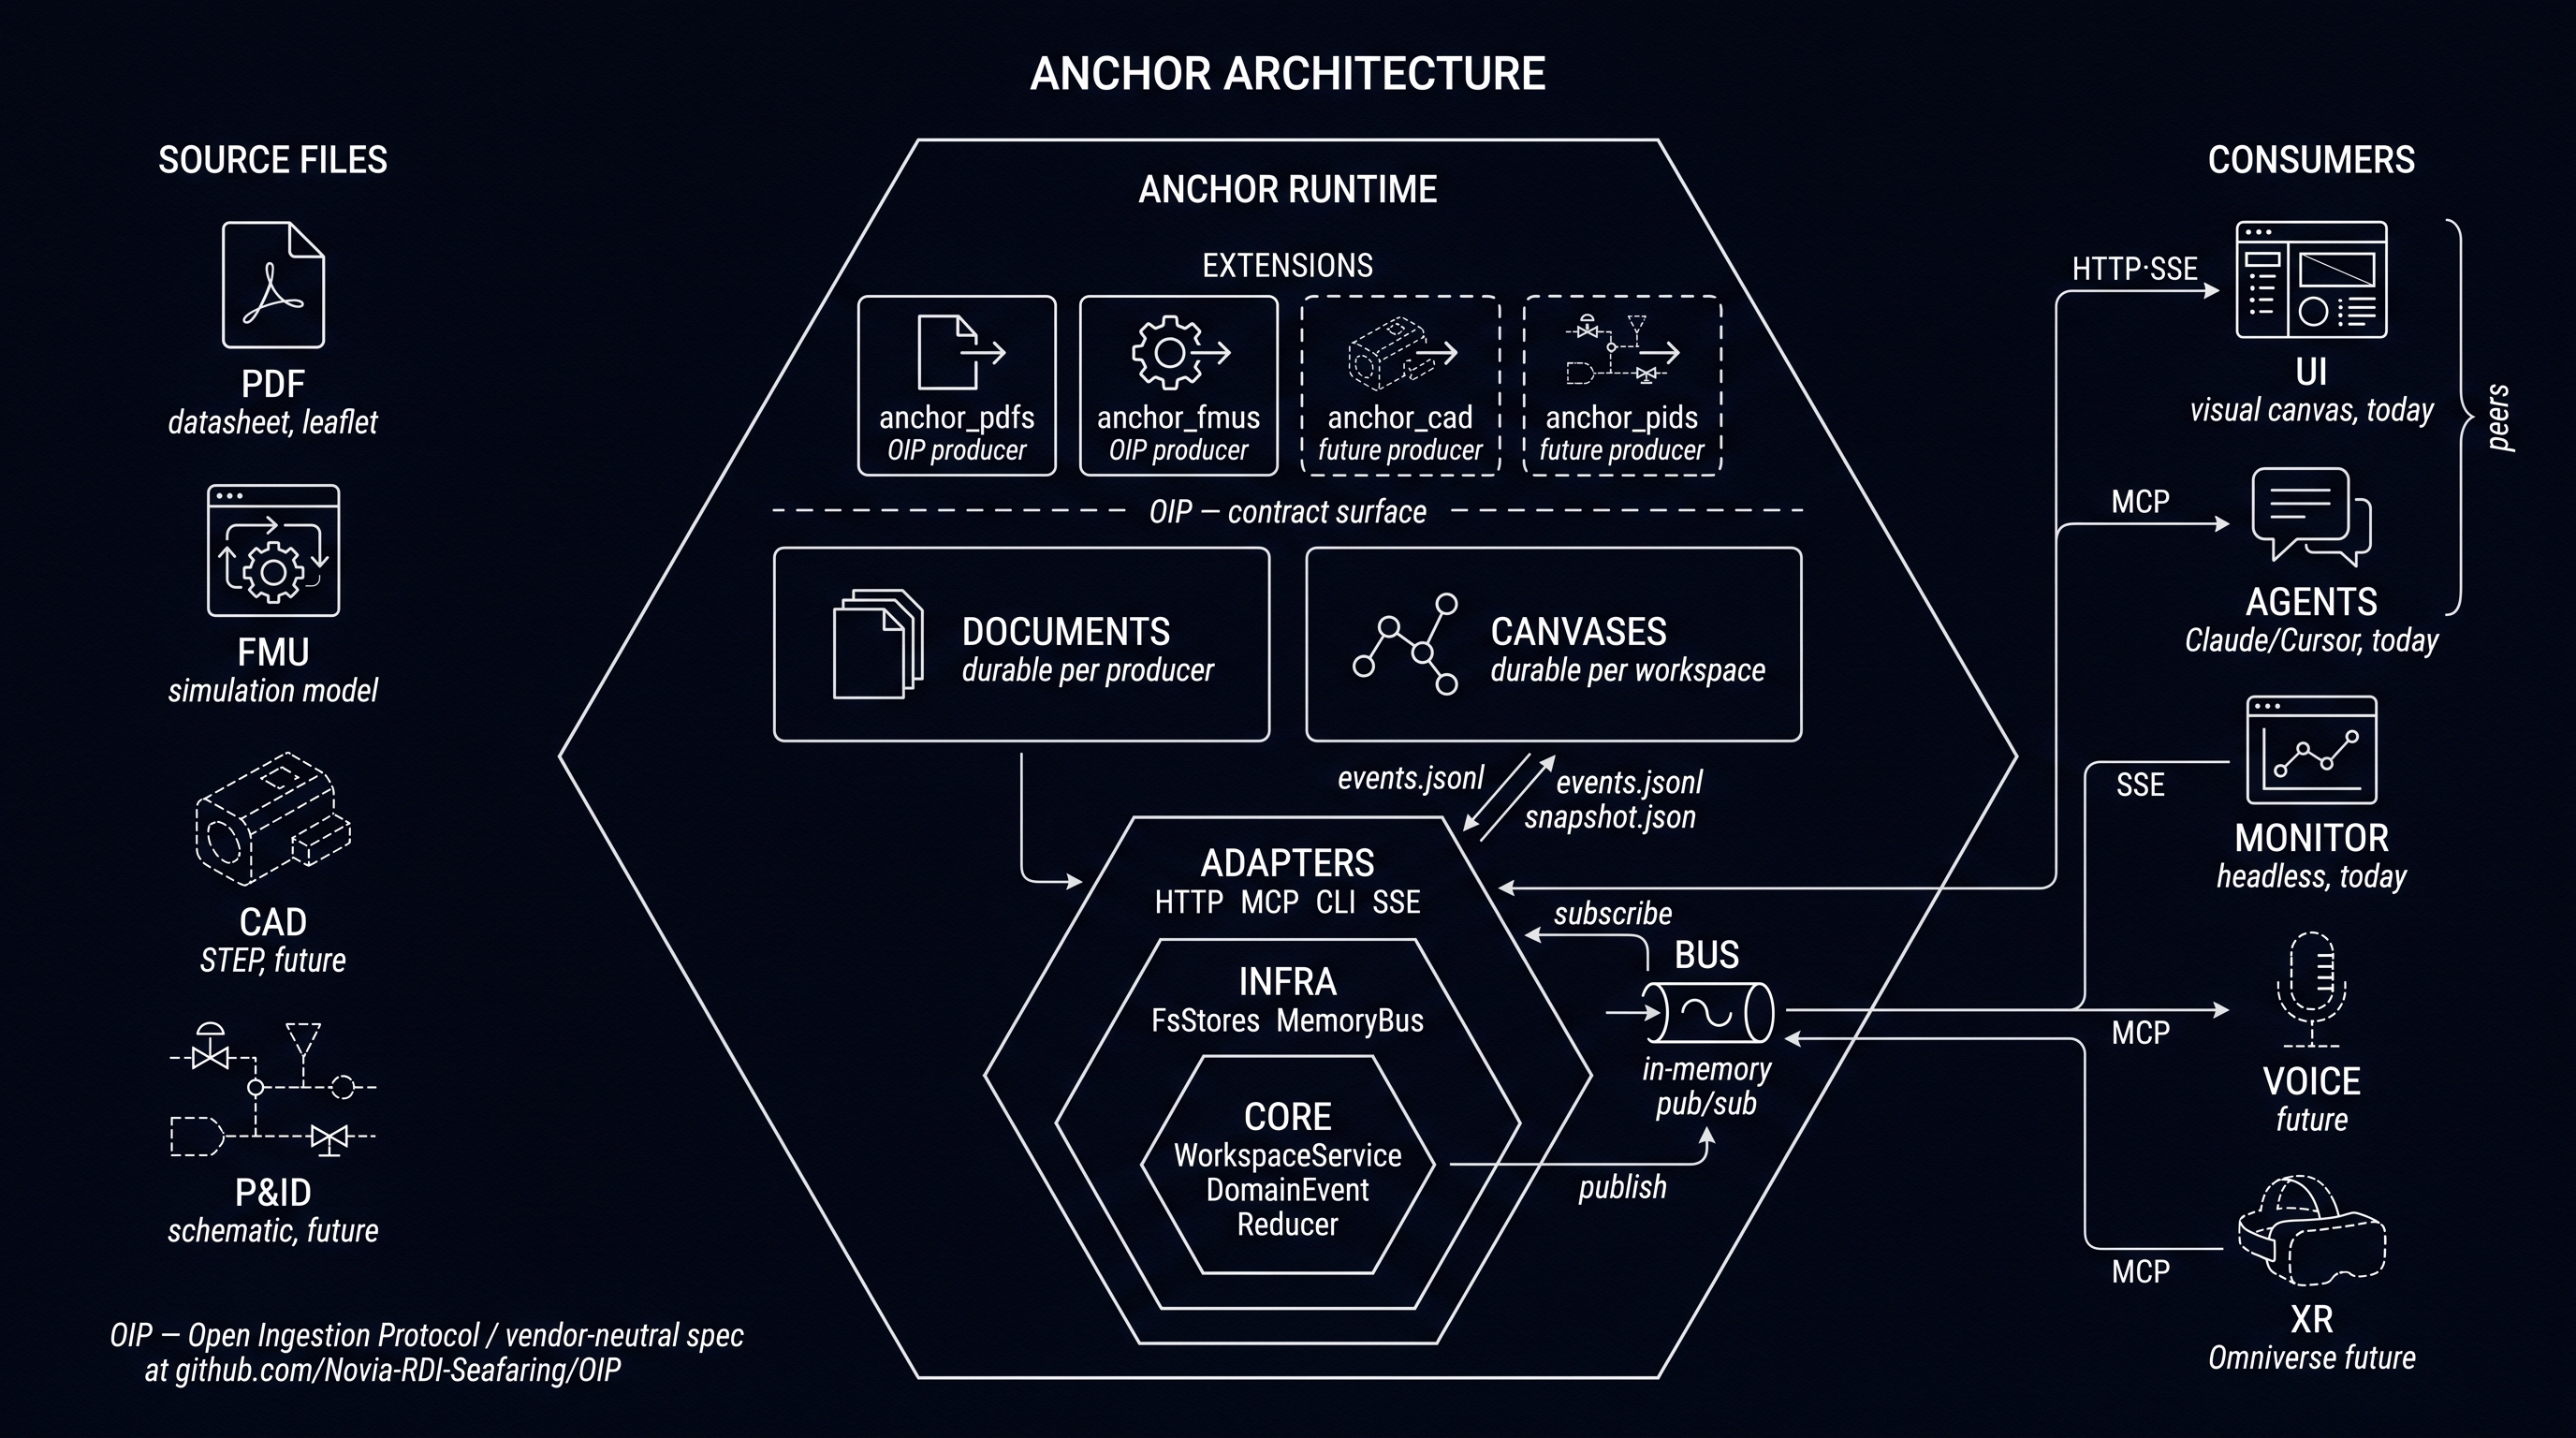
\includegraphics[width=380mm]{architecture-diagram-v16-inverted.png}
\end{textblock}

% Diagram caption (sits just above the funding line)
\begin{textblock}{443}(199,560)
  \color{centermuted}\centering
  \fontsize{10.5pt}{13pt}\selectfont
  Sources \arr{} producers \arr{} durable artefacts \arr{} core \arr{} consumers.
  Producers and consumers are pluggable; the core stays small.
\end{textblock}

% Funding line at bottom of centre column
\begin{textblock}{443}(199,580)
  \color{centermuted}\centering
  \fontsize{11pt}{14pt}\selectfont
  Funded by Business Finland · Co-Innovation Project Virtual Sea Trial · virtualseatrial.fi\\
  Novia UAS · Åbo Akademi University
\end{textblock}

% ---------------------------------------------------------------------
%  RIGHT COLUMN — graphical abstract + industry value + QR
% ---------------------------------------------------------------------
\begin{textblock}{157}(670,\contentTop)   % rightColX (656) + panelPad (14)
  \color{paneltext}\fontsize{11pt}{15pt}\selectfont\RaggedRight

  \panelhead{The canvas}
  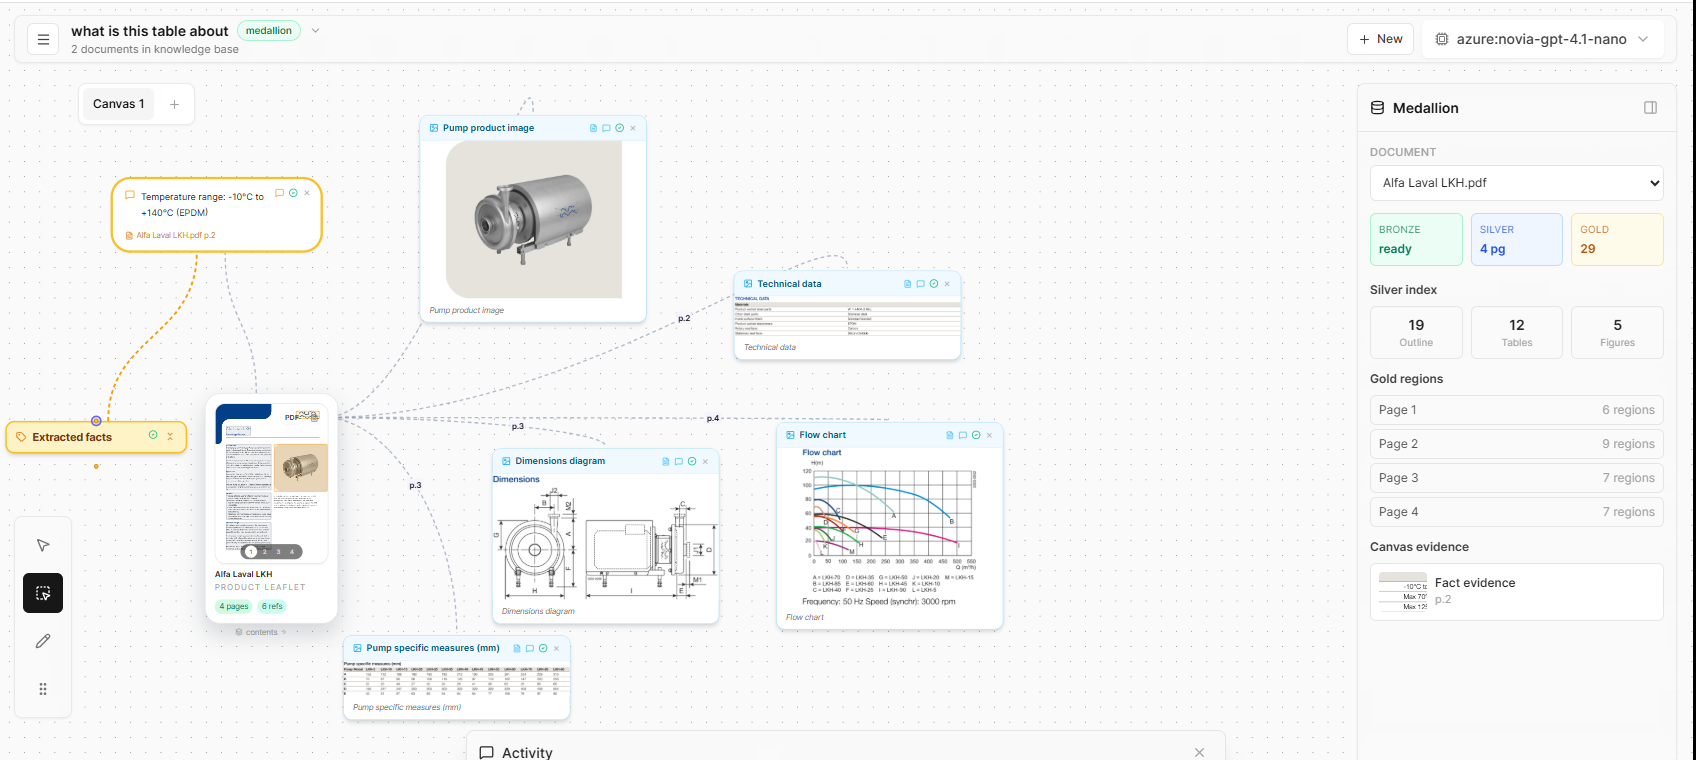
\includegraphics[width=\linewidth]{grounded_canvas.png}
  \vspace{1mm}
  {\fontsize{8.5pt}{11pt}\selectfont\color{panelmuted}
   Cards carry source crops with a one-click jump back to the PDF page. Drop a file
   onto the canvas and the producer that claims its kind ingests it in place.\par}

  \panelhead{Extensions}
  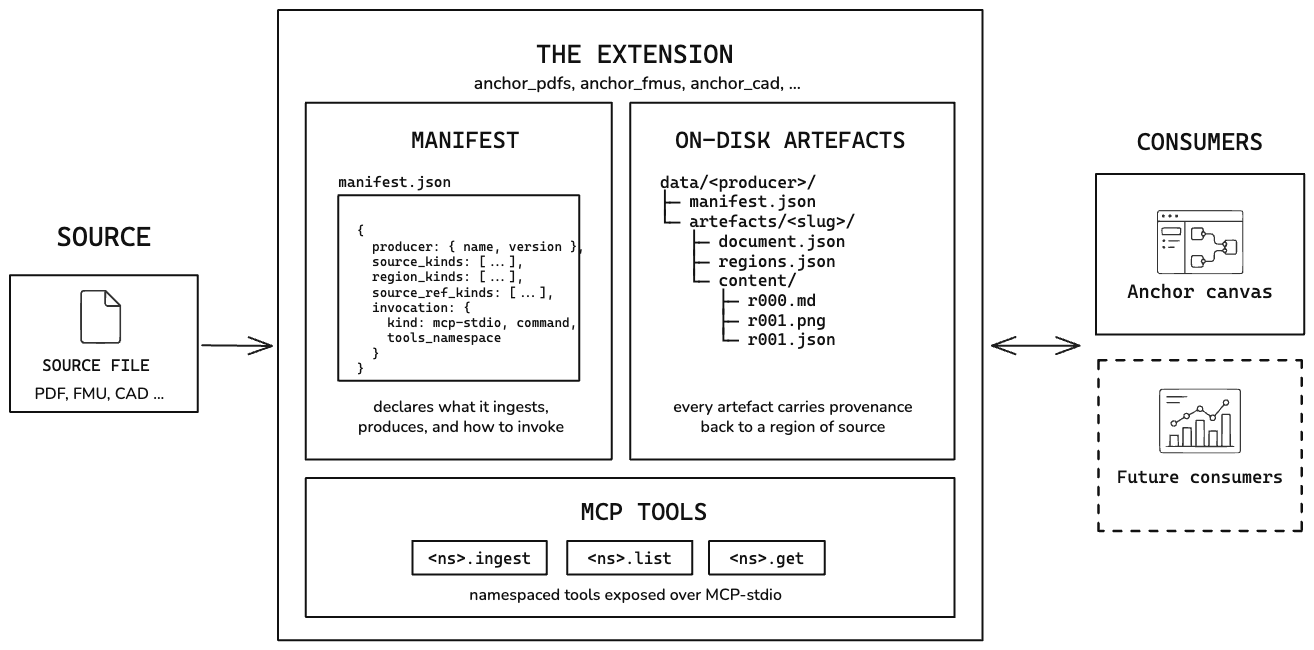
\includegraphics[width=\linewidth]{oip-arch.png}
  \vspace{1mm}
  {\fontsize{8.5pt}{11pt}\selectfont\color{panelmuted}
   An OIP extension is three things: a manifest, on-disk artefacts, and MCP tools.
   The shipped PDF producer is the working example; anything that satisfies the
   contract plugs in the same way.\par}

  \panelhead{Bring your own harness}
  The UI, MCP agents, and a CLI share one WorkspaceService and one event bus; humans
  and agent harnesses drive the canvas through identical paths. New interfaces
  (voice, XR, a chat monitor) plug in the same way.

  \panelhead{Read more}
  \vspace{1mm}
  \begin{center}
    \qrcode[height=38mm]{https://github.com/Novia-RDI-Seafaring/anchor}
  \end{center}
  \vspace{1mm}
  {\centering\fontsize{9.5pt}{12pt}\selectfont
   github.com/Novia-RDI-Seafaring/anchor\par}
  \vspace{1mm}
  {\centering\fontsize{8.5pt}{11pt}\selectfont\color{panelmuted}
   Source code and local setup instructions.\par}
  \vspace{2mm}
  \vfill
  {\color{panelmuted}\fontsize{8.5pt}{11pt}\selectfont
   Industry presentation · Vaasa, 2026\par}
\end{textblock}

\end{document}
